\section{Specifying TGG rules}

After declaring our correspondence types in the TGG schema, we can now specify a set of \emph{TGG rules} to describe the simultaneous evolution of both source, correspondence and target models.

A TGG rule is quite similar to an SDM storypattern\footnote{If you are not familiar with modelling SDMs in EA see Chapter \ref{sec:sdm_intro}} and is also of the form (\emph{precondition, postcondition}).
In other words, we have to state:
\begin{itemize}
  \item What pattern must be matched, i.e, under which conditions can the rule be applied (this is the precondition).
  \item The objects and links to be created when the rule is applied to a match (this is deduced from the postcondition).
\end{itemize}

Note that the rules of a TGG only describe the simultaneous \emph{build-up} of the models and do not delete or modify any existing elements, i.e., TGG rules are \emph{monotonic}.
This might seem surprising at first and you might think this is a terrible restriction.
The point is that the TGG should only specify a consistency relation and not directly the forward and backward transformations, which are derived automatically.
It turns out that deletion is not necessary on this level to do this, but will of course be used at the right places in the generated transformations.

\begin{enumerate}
\item[$\blacktriangleright$] In EA, open the diagram of the \texttt{Rules} package in our TGG project.
This package was generated automatically when we first created our TGG project and contains all TGG rules.

\item[$\blacktriangleright$] Create a \texttt{Rule} via drag\,\&\,drop from the TGG toolbox and set its name to \texttt{BoxToDictionaryRule} (Fig.~\ref{fig:create_tgg_rule}).

\begin{figure}[htbp]
\begin{center}
  \includegraphics[width=\textwidth]{pics/tggBilder/tggRule/tgg8}
  \caption{Creating a TGG rule}
  \label{fig:create_tgg_rule}
\end{center}
\end{figure}

\end{enumerate}

As depicted in Fig.~\ref{fig:first_tgg_rule}, the newly created rule has a method and contains a diagram (indicated by two small linked circles at the bottom right).

\begin{figure}[htbp]
\begin{center}
  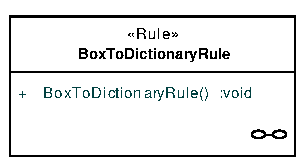
\includegraphics[width=0.35\textwidth]{pics/tggBilder/tggRule/tgg9}
  \caption{Our first TGG rule}
  \label{fig:first_tgg_rule}
\end{center}
\end{figure}

\begin{enumerate}
\item[$\blacktriangleright$] Double click \texttt{BoxToDictionaryRule} to open its diagram.

\item[$\blacktriangleright$] Drag\,\&\,drop a \texttt{Box} from the project browser, this time to create an instance of \texttt{Box}, and enter \texttt{box} as its name.
Choose \texttt{Create} as binding operator (Fig.~\ref{fig:create_tgg_object}).

\begin{figure}[htbp]
\begin{center}
  \includegraphics[width=\textwidth]{pics/tggBilder/tggRule/tgg10}
  \caption{Creating an object variable in a TGG rule}
  \label{fig:create_tgg_object}
\end{center}
\end{figure}

\item[$\blacktriangleright$] In the same way, create \texttt{dictionary} as an instance of \texttt{Dictionary}.

\item[$\blacktriangleright$] Also create \texttt{boxToDictionary} as an instance of the correspondence type \texttt{BoxToDictionary}, by using Quick-Link between \texttt{box} and \texttt{dictionary} and choosing ``Create TGG Correspondence Link'' (Fig. \ref{fig:create_tgg_correspondence_link}).

\begin{figure}[htbp]
\begin{center}
  \includegraphics[width=\textwidth]{pics/tggBilder/tggRule/create_tgg_correspondence_link.png}
  \caption{Creating a TGG correspondence link via Quick-Link}
  \label{fig:create_tgg_correspondence_link}
\end{center}
\end{figure}
\FloatBarrier

\end{enumerate}

Our current rule creates a box, a dictionary, and an appropriate correspondence all at the same time.

But how about the \texttt{name} of the box and the \texttt{title} of the dictionary?
\note{Attribute Constraints}
We use \emph{attribute constraints} in TGG rules to provide a bidirectional and high-level solution for attribute manipulation.
In this case we need a constraint which ensures that \texttt{box.name} and \texttt{dictionary.title} are set to the same value.

\begin{enumerate}
  \item[$\blacktriangleright$] To create such a constraint, drag\,\&\,drop a \emph{TGG Constraint} from the \texttt{TGGRuleTolboxPage} (Fig.~\ref{fig:common_toolbox}).

  \begin{figure}[htbp]
  \begin{center}
    \includegraphics[width=0.25\textwidth]{pics/tggBilder/tggRule/tgg12}
    \caption{Constraint from the Toolbox in EA}
    \label{fig:common_toolbox}
  \end{center}
  \end{figure}

  \item[$\blacktriangleright$] Double click the constraint element to open it, choose ``eq'' under ``Constraints'', enter the values depicted in
  Fig.~\ref{fig:first_tgg_constraint} and add the constraint.
  Affirm with \texttt{OK}.

  \begin{figure}[htbp]
  \begin{center}
    \includegraphics[width=0.7\textwidth]{pics/tggBilder/tggRule/tgg13.png}
    \caption{Creating a Constraint in EA}
    \label{fig:first_tgg_constraint}
  \end{center}
  \end{figure}

  \item[$\blacktriangleright$] Quick-link a \texttt{Dependency} from the
  constraint to the involved object variables, \texttt{box} and \texttt{dictionary}.
  The rule should now resemble Fig.~\ref{fig:tgg_rule_with_constraint}.

  \begin{figure}[htbp]
  \begin{center}
    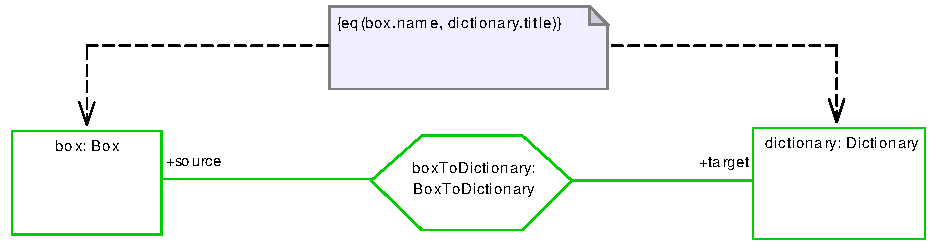
\includegraphics[width=\textwidth]{pics/tggBilder/tggRule/tgg14}
    \caption{A TGG Rule with a Constraint}
    \label{fig:tgg_rule_with_constraint}
    \end{center}
  \end{figure}

\end{enumerate}

To complete our first TGG rule, we still need to create the initial structure of a learning box.
In contrast to the rather simple dictionary, where \texttt{Dictionary} is a direct container for \texttt{Entry} objects, we have to create a number of connected \texttt{Partitions} that hold the \texttt{Cards} in the learning box.

\begin{enumerate}
  \item[$\blacktriangleright$] Create three \texttt{Partition} object variables with all appropriate links, so that your TGG rule diagram closely resembles Fig.~\ref{fig:boxtodictionaryrule_complete}.

  \begin{figure}[htbp]
  \begin{center}
    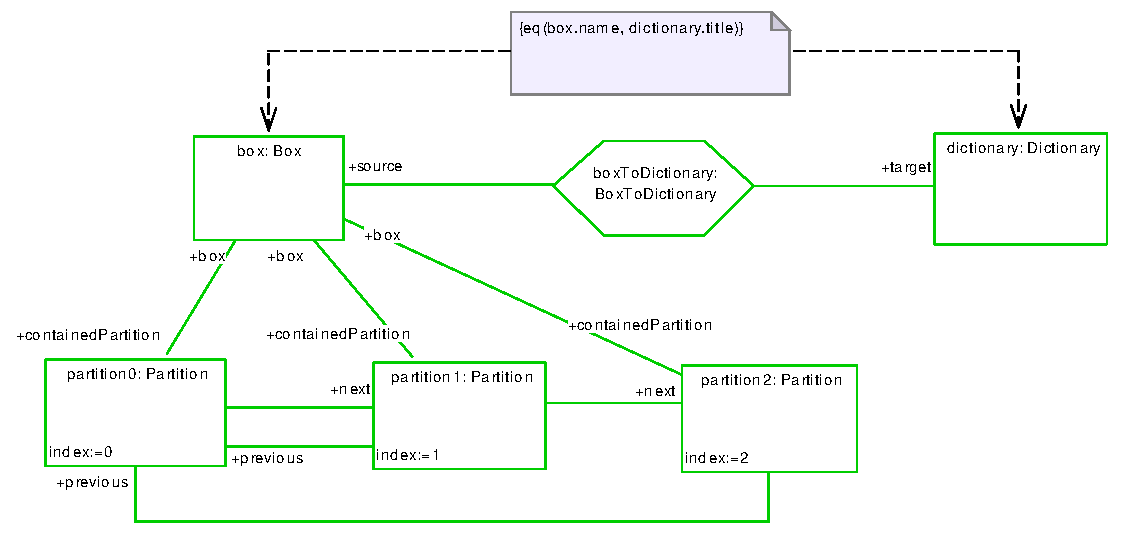
\includegraphics[width=\textwidth]{pics/tggBilder/tggRule/tgg15}
    \caption{Complete TGG rule diagram for \texttt{BoxToDictionaryRule}}
    \label{fig:boxtodictionaryrule_complete}
  \end{center}
  \end{figure}

\end{enumerate}

If you are in hurry, you may already proceed to Sect.~\ref{sect:TGGs_in_Action} and transform a box to a dictionary and vice-versa.
But please be aware that your specified TGG (with just one rule) will only be able to cope with empty boxes and dictionaries.
Handling additional elements (cards in the learning box and entries in the dictionary) requires a second rule \ldots

To create the second rule, we will introduce another method. Note that both methods generate the same results and the following one is only a shortcut.

\begin{enumerate}
  \item[$\blacktriangleright$] Select \texttt{box}, \texttt{boxToDictionary}, \texttt{dictionary} and \texttt{partition0} in \texttt{BoxToDictionaryRule}.
  \item[$\blacktriangleright$] Choose ``Derive'' in the ``eMoflon TGG Functions'' section of the add-in window as depicted in Fig. \ref{fig:derive_from_tgg_rule} (if you cannot see this window, make sure ``Extensions $\rightarrow$ Add-In Window'' is activated) and enter ``CardToEntryRule'' as the name in the dialog that shows up. This will generate a new rule which already contains the elements it is derived from.

  \begin{figure}[htbp]
  \begin{center}
    \includegraphics[width=0.6\textwidth]{pics/tggBilder/tggRule/derive_tgg_rule.png}
    \caption{Derive from an existing TGG rule}
    \label{fig:derive_from_tgg_rule}
  \end{center}
  \end{figure}
  \FloatBarrier

  \item[$\blacktriangleright$] Add instances of \texttt{Card} and \texttt{Entry} to the rule and add links until the diagram closely resembles Fig. \ref{fig:cardtoentry_1}.

  \begin{figure}[htbp]
  \begin{center}
    \includegraphics[width=\textwidth]{pics/tggBilder/tggRule/tgg19}
    \caption{\texttt{CardToEntryRule} without attribute manipulation}
    \label{fig:cardtoentry_1}
  \end{center}
  \end{figure}

\end{enumerate}


As a final step, we now have to specify how attributes are to be handled via appropriate attribute constraints.

The \texttt{content} of an \texttt{Entry} in a \texttt{Dictionary} is to be of the form \texttt{<word> : <meaning>}, while the \texttt{face} of a \texttt{Card} must read \texttt{Question: <word>}, and the \texttt{back} \texttt{Answer: <meaning>}.

Using two predefined attribute constraint \texttt{addPrefix} and \texttt{concat}, we can specify this as a set of constraints:

\begin{enumerate}
\item[$\blacktriangleright$] Add a new constraint to your diagram with the following three lines:
\begin{quotation}
\noindent \texttt{addPrefix("Question: ", word, card.face)}\\
\texttt{addPrefix("Answer: ", meaning, card.back)}\\
\texttt{concat("~:~", word, meaning, entry.content)}
\end{quotation}

\end{enumerate}

After connecting appropriatly, your rule should now resemble Fig.~\ref{fig:cardtoentry_2}.

\begin{figure}[htbp]
\begin{center}
  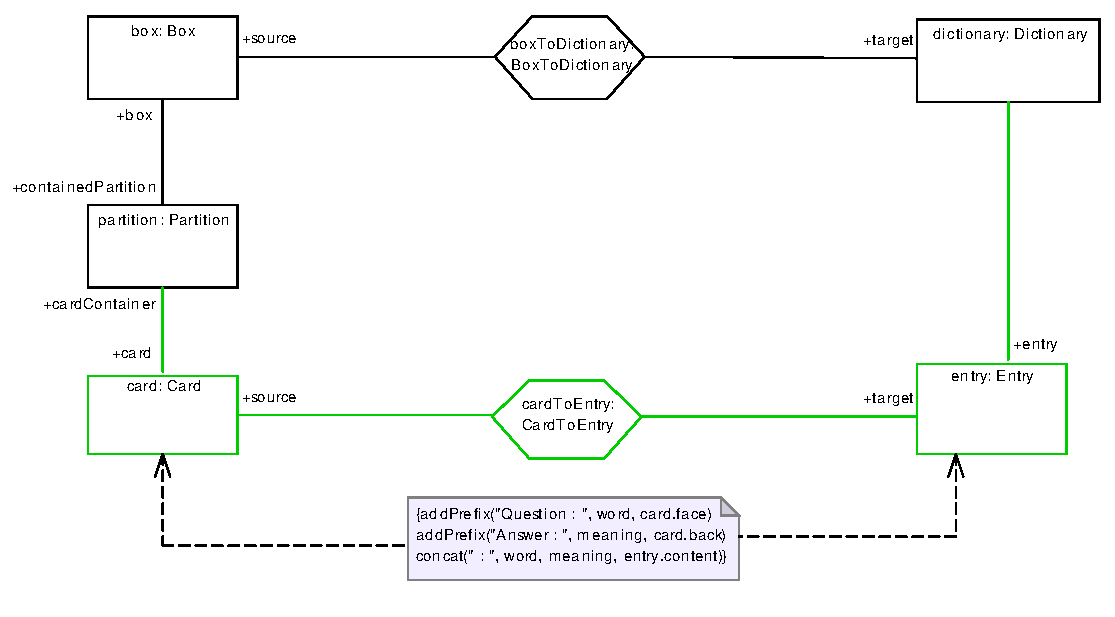
\includegraphics[width=\textwidth]{pics/tggBilder/tggRule/tgg20}
  \caption{Attribute manipulation for \texttt{card} and \texttt{entry}}
  \label{fig:cardtoentry_2}
\end{center}
\end{figure}
\FloatBarrier

Finally, we have to specify how the partition, into which the newly created card is to be placed, must be chosen.
We shall implement the following simple rule: a card in a partition with index 0/1/2 corresponds to an \texttt{Entry} of level beginner/advanced/master.
This time, we must define our very own attribute constraint to handle this mapping.
For the moment, we are just going to declare and use the attribute constraint, which will be implemented later in Java.


\begin{enumerate}
\item[$\blacktriangleright$] Add a further constraint to your diagram, but this time do not choose a predefined constraint but click ``Add'' below the dropdown menu and enter the values given in Fig. \ref{fig:create_new_constraint}.

\begin{figure}[htbp]
\begin{center}
  \includegraphics[width=0.55\textwidth]{pics/tggBilder/tggRule/create_new_constraint}
  \caption{Create a user defined constraint.}
  \label{fig:create_new_constraint}
\end{center}
\end{figure}
\FloatBarrier

\item[$\blacktriangleright$] After saving this new constraint, choose it and enter the given values:

\begin{quotation}
\texttt{indexToLevel(partition.index, entry.level)}
\end{quotation}
\end{enumerate}

After defining the dependencies of the constraint, your complete TGG rule should resemble Fig.~\ref{fig:cardtoentry_complete}.
\begin{figure}[htbp]
\begin{center}
  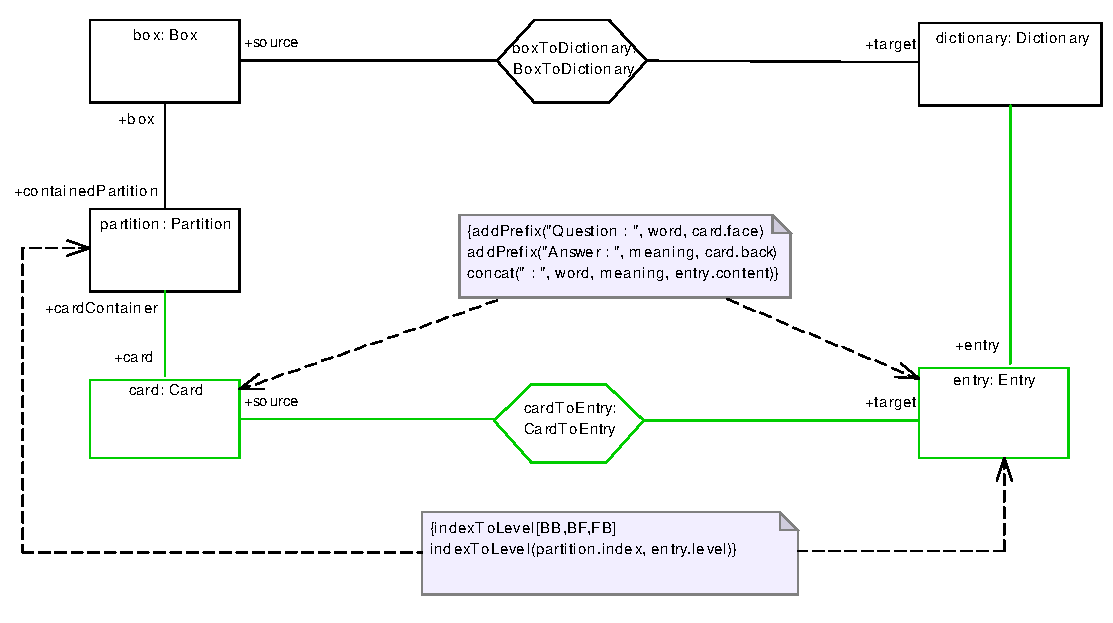
\includegraphics[width=\textwidth]{pics/tggBilder/tggRule/tgg21}
  \caption{\texttt{CardToEntryRule} with complete attribute manipulation}
  \label{fig:cardtoentry_complete}
\end{center}
\end{figure}

Just like the patterns describing \emph{structural} correspondence,  attribute constraints can be automatically \emph{operationalized} as required for the concrete transformations (forward, backward).
Even more interesting, a set of constraints might have to be ordered a bit differently depending on the direction of the transformation, and some constraints might have to be checked for already set attributes, while others must set values appropriately to fulfill the constraint.

For built-in or \emph{library} constraints (Appendix
~\ref{chap:libraryConstraints}) such as \emph{eq}, \emph{addPrefix} and
\emph{concat}, you do not need to worry about these details and can just express what should hold -- everything is handled automatically.

In many cases, however, a constraint might be very problem-specific, such as our \emph{indexToLevel} constraint, and there might not be any fitting combination of library constraints to express the consistency condition.

In such a case, the new attribute constraint must be declared before its use.

The list of \emph{adornments} in the declaration specifies the cases for which the constraint can be operationalized.
Each adornment consists of a \texttt{B} for bound or an \texttt{F} for free, for each argument of the constraint.
This is much simpler than its sounds so lets take a look at our example:
\begin{description}
\item[BB] means that the \texttt{partition.index} and \texttt{entry.level} can both be \emph{bound}, i.e., already have assigned values.
In this case, the \emph{operation} (the operationalized constraint) must check if the assigned values are correct.
\item[BF] means that \texttt{partition.index} is \emph{bound} and \texttt{entry.level} is \emph{free}, i.e., the operation must determine and assign the correct value to \texttt{entry.level} using \texttt{partition.index}.
\item[FB] means that \texttt{partition.index} is \emph{free} and \texttt{entry.level} is \emph{bound}, i.e., the operation must determine and assign the correct value to \texttt{parti\-tion.in\-dex} using \texttt{entry.level}.
\end{description}

Note that we decide not to support \textbf{FF} as we would have to generate a consistent pair of index and level.
Although this is possible and might even make sense for some applications, in our case it does not (the pair is not unique\ldots which pair should we take?).

At compile time, the set of constraints (also called \emph{Constraint Satisfaction Problem} (CSP)) for every TGG rule is ``solved'' for each case (forward, backward) by operationalizing all constraints and determining a feasible (compatible to the declared adornments of each constraint) sequence in which the operations can be executed.
An exception is thrown if this is not possible.
